% fancytikzposter.tex, version 2.1
% Original template created by Elena Botoeva [botoeva@inf.unibz.it], June 2012
% 
% This file is distributed under the Creative Commons Attribution-NonCommercial 2.0
% Generic (CC BY-NC 2.0) license
% http://creativecommons.org/licenses/by-nc/2.0/ 


\documentclass{a0poster}

\usepackage{fancytikzposter} 
\usepackage{fancySettings} 
\usepackage{mystyle}


\title{Parallel Tempering \qquad }
\author{ dr Błażej Miasojedow \and \udot{mgr Mateusz Łącki} \\
  Wydział Matematyki, Informatyki i Mechaniki\\ University of Warsaw, Poland\\
  \texttt{B.Miasojedow@mimuw.edu.pl} \\
  \texttt{mateusz.lacki@biol.uw.edu.pl}
}

\usetemplate{1}

\begin{document}

\ClearShipoutPicture
\AddToShipoutPicture{\BackgroundPicture}

\noindent % to have the picture right in the center
\begin{tikzpicture}
  \initializesizeandshifts
  % \setxshift{15}
  % \setyshift{2}


  %% the title block, #1 - shift, the default value is (0,0), #2 - width, #3 - scale
  %% the alias of the title block is `title', so we can refer to its boundaries later
\ifthenelse{\equal{\template}{1}}{ 
  \titleblock{47}{1}
}{
  \titleblock{47}{1.5}
}


  %% #1 - anchor relative to the title block, #2 - shift, #3 - width, #3 - file name
\addlogo[south west]{(2,1.5)}{8cm}{img/logoUniversityOfWarsaw.png}
% \addlogo[south east]{(-2,1.5)}{16cm}{img/logoMimuw.png}

\blocknode{Bayesian Inference}{
  \coloredbox{colorthree!50!}{\centering Classical Inference}
  \bi
    \item{Hierarchical modelling}
  \ei
  \coloredbox{colorthree!50!}{\centering Model Selection}  

}
  
\blocknode{Picture}{
  \begin{tikzfigure}[Metropolis Hastings]
    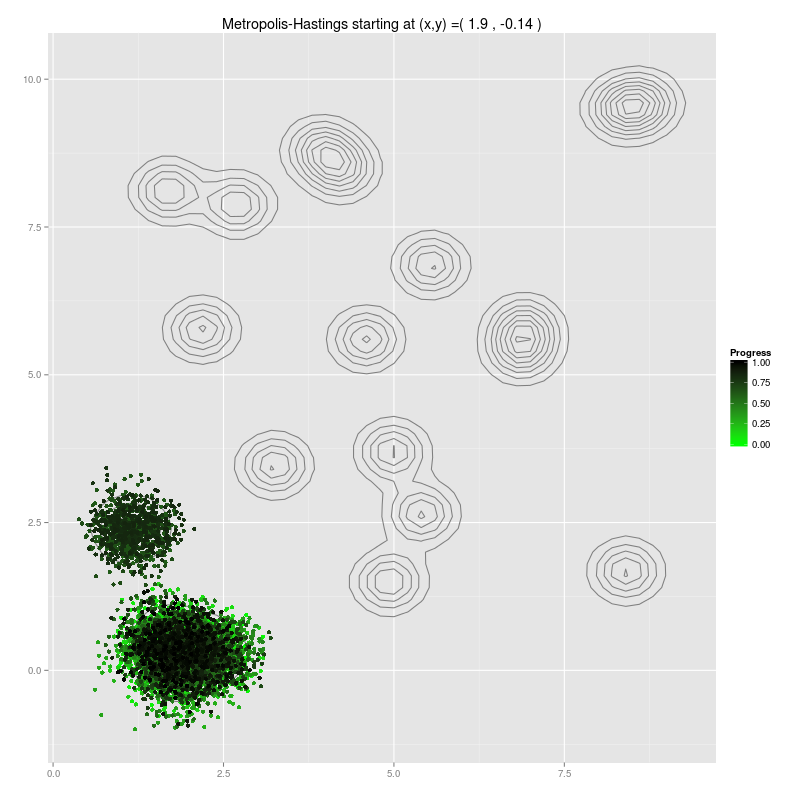
\includegraphics[scale=1]{img/MH_simululation_10000_steps.png}
  \end{tikzfigure}
} 

\startsecondcolumn
\blocknode{Middle}{Middlearth}

\startthirdcolumn
\blocknode{Bye}{
bkas
  Bye World \citet{Medvedovic}
}

\blocknode{References}{
  \bibliographystyle{bibliography/eccaNoNotes}
  \tiny{ 
    \bibliography{bibliography/references}
  }
}

\end{tikzpicture}


\end{document}




